\subsection{Water governance regimes}
\label{Res.1}

\begin{figure}[ht!]
	\centering
	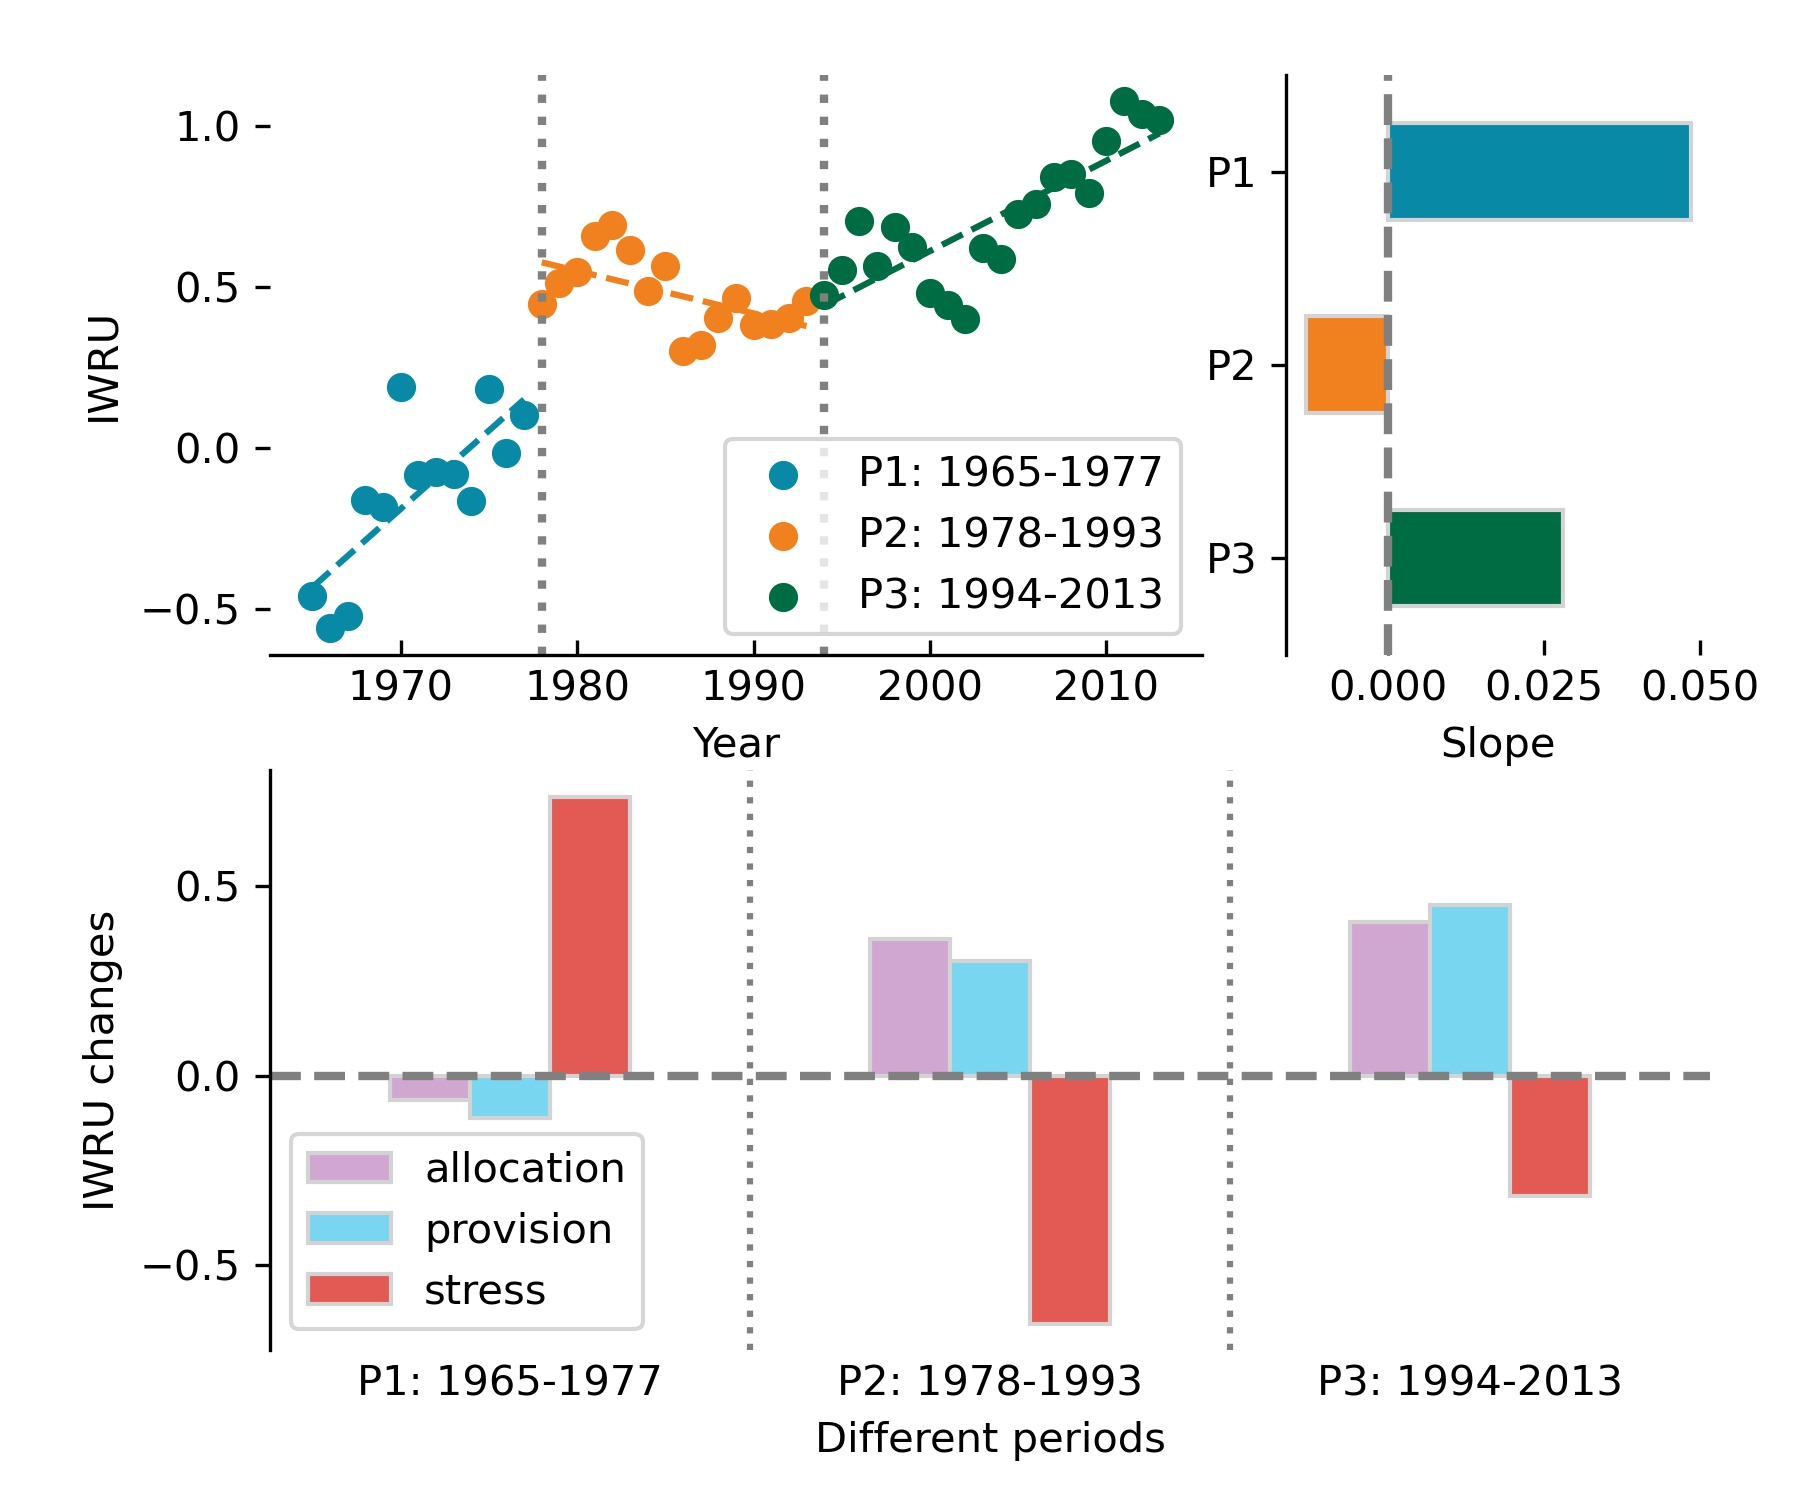
\includegraphics[width=0.9\linewidth]{main/index.jpg}
	\caption{Changes in the IWGI index. 
	\textbf{A,} Change points detection. With significant change points in 1978 and 1994, the IWGI has three different periods.
	\textbf{B,} Contributions of each dimension to the changes of IWGI within each of the three periods. Supply, purpose and allocation were respectively the main positive contributors to P1, P2 and P3.
	}
	\label{fig:IWGI}
\end{figure}

% 这一节主要展示IWGI的变化趋势和WUR的划分
With two significant breakpoints, the changes in the IWGI are divided into three periods (Figure~\ref{fig:IWGI}A) with different slopes. 
The changes are contributed by different water governance dimensions (Figure~\ref{fig:IWGI}B).
% 第一阶段
In the first period (P1, 1965-1978), the IWGI increased rapidly. 
Water supply made the most striking positive contribution (131\%), while purpose and allocation had a slight negative contribution (-11\% and -20\%).
% 第二阶段
In the second period (P2, 1979-1994), the contributions of purpose and allocation became positive and the IWGI experienced a drop because steeply declining supply capacity played a larger negative role (dropping to -188\% lower than P1). 
% 第三阶段
In the third period (P3, 1995-2013), as positive contributions from purpose (75\%) and allocation (84\%) increased further and the negative contribution of water supply lessened (-59\%), positive growth of the IWGI returned.

% 每个时期都有一个独特的、最引人注目的、对IWGI作出积极贡献的人。不同时期的三维总体特征如图所示。
Each period has a unique most striking contributor to IWGI in positive. Overall features of the three dimensions in different periods are shown in Figure~\ref{fig:phases}.
% 第一阶段到第二阶段
Throughout P1, the water governance regime was dominated by increasing supply capacities. 
% 第三阶段集中
It then experienced a shift, slowing down in increasing supply during P2, with an accompanying reverse in the contributed proportion between purpose and allocation. Finally, the contribution of all three dimensions was similar in P3 (32.91\%, 31.87\% and 35.21\% for purpose, allocation and supply respectively), making the points cluster at the centre of the diagram. 
% 总结来说,三个稳态
The three different periods corresponded to three distinct water governance regimes: a massive supply regime (P1: 1965-1978), a purpose-focused regime (P2: 1979-1993), and a many-sided governance regime (P3: 1994-2013). 


\begin{figure}[!htbp]
	\centering
	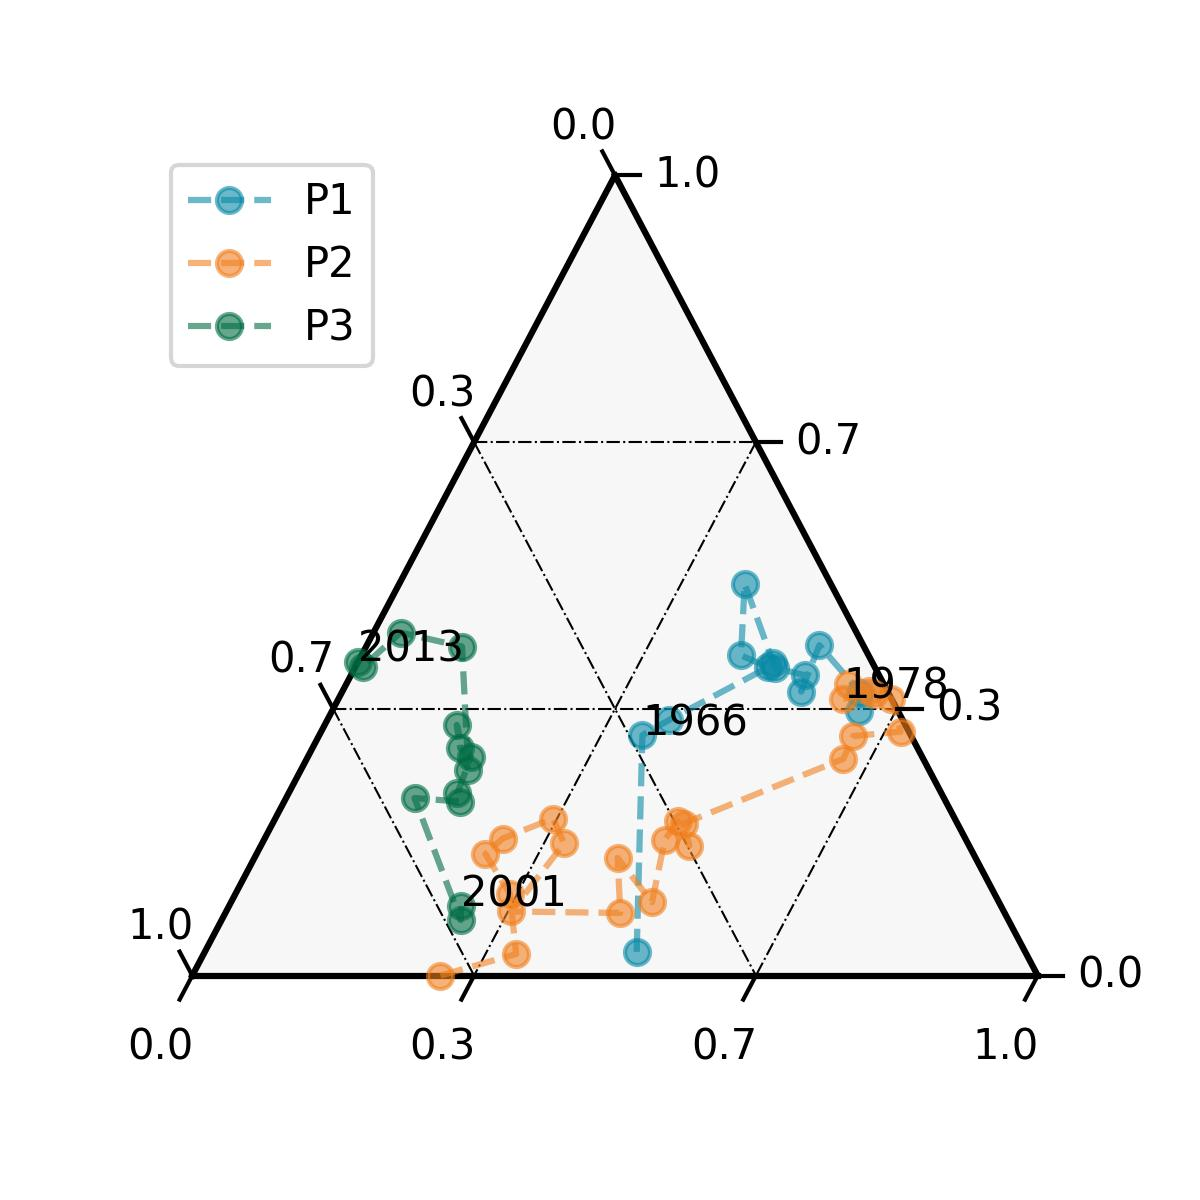
\includegraphics[width=0.9\linewidth]{main/phases.jpg}
	\caption{Combination of contributions across three dimensions in different periods (S: supply; P: purpose; A: allocation). The closer a point is to an angle of the outside triangle, the greater the proportion of the contribution of this dimension.
	The red indicator line in this plot denotes a 1:1 contributions between purpose (P) and allocation (A). When the points are below this line, the contribution ratio of allocation is lower than that of function, and \textit{vice versa}.}
	% 由于阶段一的点位于该线上方,L的净贡献比例多于P,而第二阶段的点则恰好相反。
	\label{fig:phases}
\end{figure}

\subsection{Causes of water governance regime shifts}
\label{Res.2}

\begin{figure}[th!]
	\centering
	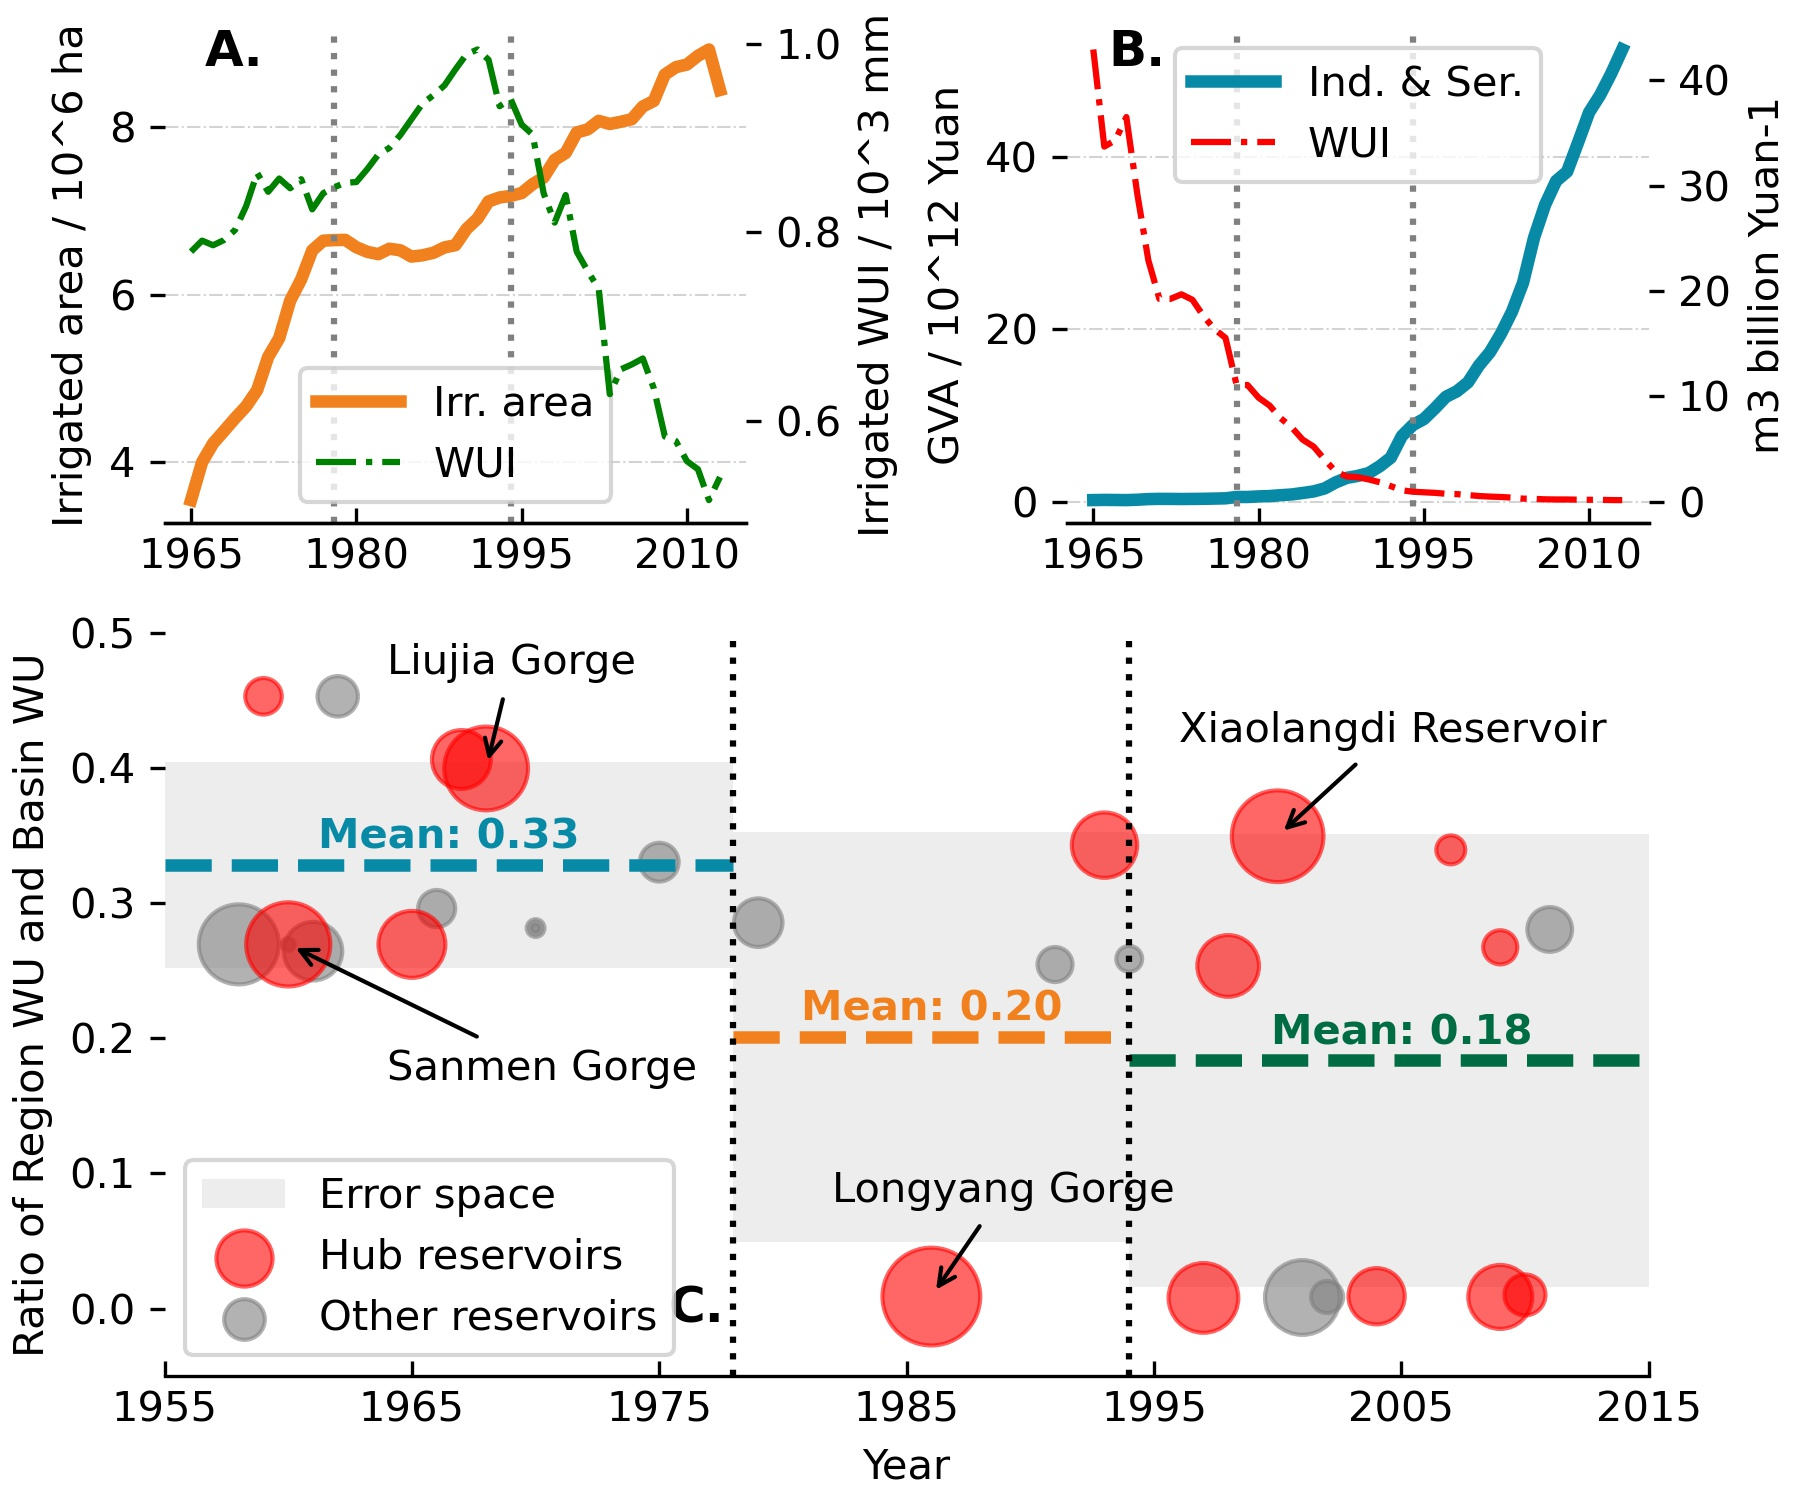
\includegraphics[width=0.9\linewidth]{main/causes.jpg}
	\caption{
		Causes of water governance regime shifts in the Yellow River Basin: environmental change, economic growth and efficiency changes, social transformation, and water governance policies.
		\textbf{A.} Changes in total irrigated area (orange line), and water uses in per unit of area (WU/A, green dot line, see \textit{SI Appendix} Methods S2).
		\textbf{B.} Changes in gross values added (GVA) of industry and services (blue line), and their water use for unit production (WU/GVA, red dot line) respectively (\textit{SI Appendix} Methods S2).
		\textbf{C.} Completed time of each new reservoir and their surrounding region's water use percentages as a proportion of the basin's total water use (WU) at that time. Red circles denote hub reservoirs in the basin, which play a role in integrated basin water management. 
		The size of each circle indicates the magnitude of its water storage capacity. Some important reservoirs include: (1) Xiaolangdi reservoir and Sanmen Reservoir, which were constructed mainly for managing sediments; and (2) Impoundments at Liujia Gorge, Longyang Gorge, which were constructed mainly for managing flood water discharge and water supply. The named reservoirs are significant for the entire basin, not only for regional development.
		\textbf{D.} Social transformations and national-level policies related to water governance (see \textit{SI Appendix} Methods S1 and Table S2). In order, the four transformations are ``ethos of conquer nature (since 1958)'', ``reform and opening-up (since 1978)'', ``the 87 Water Allocation Scheme (since 1987)'', ``environmental regulation (since 2003)'' in order (see \textit{SI Appendix} Methods S1).
	}
	\label{fig:Causes}
\end{figure}

% 进一步挖掘IWGI变化的根本原因,灌溉区扩张和工业和服务业的经济增长是P1和P2目的变化的关键。
Digging more deeply into the underlying causes of changes in the IWGI, the expansion of irrigated area and the economic growth of industry and services were key to the change in purpose between P1 and P2. 
% P1年,黄河流域灌溉农业面积以图A的速度快速扩张,灌溉用水占主导(1965年占总用水的$81.56\%$, 1978年占总用水的$83.17\%$,图S3)。
During P1, the area of irrigated agriculture in the Yellow River Basin expanded rapidly at a rate of $0.25*10^6 ha/yr$ (Figure\ref{fig:Causes} A), and irrigation water was the dominant water use ($81.56\%$ of the total water use in 1965, and $83.17\%$ in 1978 \textit{SI Appendix} Fig. S3). 
% 然而,进入P2后,灌溉区扩张停滞,工业和服务业逐渐增长,用水需求增加(图re\ref{fig: Causes} B),导致灌溉用水量比例下降$8\%$ S3。
Entering P2, however, the expansion of irrigated area stalled and industry and services gradually took off, with more water demands (Figure\ref{fig:Causes} A and B), leading to a $8\%$ reduction in the proportion of irrigation water use (\textit{SI Appendix} S3).

% 水分利用效率由P2变化到P3。
The efficiency of water use changed from P2 to P3. 
While irrigated area resumed its expansion again in P3 (Figure\ref{fig:Causes}A), industry and urban services assumed a stronger economic role (represented by Gross Added Values, GVA) (Figure~\ref{fig:Causes}B). 
However, because of more efficient technology and better water conservation practices (\textit{SI Appendix} Fig. S4), both experienced significant declines in water use for unit irrigated area or unit production (Figure~\ref{fig:Causes}A and Figure~\ref{fig:Causes}B). 
As a result, the differences between sectors of water use were reduced while the total water consumption remained stable during P3 (\textit{SI Appendix} Fig. S3).

% 最后,环境背景、社会转型和水治理政策在这三个时期都发挥了作用。
Finally, environmental context, social transformation and water governance policies played roles in all three regimes. 
% 我们计算了每个水库的区域和盆地用水比例(R/B ratio),较高的比例代表潜在的供水作用,而不是调节作用。
We calculated the ratios of regional and basinal water use for each reservoir (R/B ratio), with a higher ratio representing a potential role for supply rather than regulation (Figure~\ref{fig:Causes}C).
% 在自然水资源相对丰富的P1年,水库大多建在需水量高的地区,水库的需水量比显著偏高。
Under the guiding ethos of ``conquering nature'', most of the reservoirs were built in regions with high water demands during P1, when natural water resources were relatively abundant (\textit{SI Appendix} Fig. S5), and R/B ratios were significantly higher (Figure~\ref{fig:Causes}C, p<0.01). 
% 在P2中,新水库的数量显著减少,水量分配受到“87调水方案”的严格控制,总库容几乎没有增加(\textit{SI  Appendix}图S6)。
In P2, the number of new reservoirs decreased significantly and allocation of water was rigorously controlled by ``the 87 Water Allocation Scheme'', with little increase in total water storage capacity (\textit{SI Appendix} Fig. S6). 
% 进入P3期后,以“环境监管”为指导的无数国家层面的水治理政策被提出,为了便于监管,新建的水库数量甚至更多,其中大部分建在R/B比较低的地区。
Entering P3, myriad national-level water governance policies were proposed under the guide of ``environmental regulation'' (Figure~\ref{fig:Causes}D), and the number of new reservoirs was even higher for facilitating and regulating objectives. Most of these were built in regions with lower R/B ratios (Figure~\ref{fig:Causes}C and \textit{SI Appendix} Fig. S6).

